% ============================================================
% GeoSignal: An Offline Historical Replay of a Proposed
% Geopolitical Monitoring Workflow
% Generic article class -- swap in the venue template (e.g. AAMCT)
% once it is available. Search for \todo{} to find open items.
% ============================================================
\documentclass[10pt,a4paper,twocolumn]{article}

\usepackage[utf8]{inputenc}
\usepackage[T1]{fontenc}
\usepackage{lmodern}
\usepackage[margin=1.8cm]{geometry}
\usepackage{microtype}
\usepackage{amsmath,amssymb}
\usepackage{booktabs}
\usepackage{array}
\usepackage{graphicx}
\usepackage{xcolor}
\usepackage{caption}
\usepackage{tikz}
\usetikzlibrary{arrows.meta,positioning,shapes.geometric}
\usepackage{pgfplots}
\pgfplotsset{compat=1.17}
\usepackage[hidelinks]{hyperref}
\setlength{\columnsep}{0.65cm}

\newcommand{\todo}[1]{\textcolor{red}{[TODO: #1]}}
\newcommand{\CAR}{\mathrm{CAR}}

\title{GeoSignal: An Offline Historical Replay of a Proposed\\Geopolitical Monitoring Workflow}
\author{P. Krishna Surya\\
\small School of Advanced Sciences\\
\small VIT-AP University\\
\small Amaravati, Andhra Pradesh 522241, India\\
\small krish20041610@gmail.com}
\date{October 2026}

\begin{document}
\maketitle

% ------------------------------------------------------------
\begin{abstract}
Geopolitical developments can affect firms and markets through multiple, time-varying exposure channels, yet monitoring workflows must connect event records, reporting, economic entities, and market data before analysts can assess those channels. This paper examines whether a prototype designed for future live geopolitical monitoring can exercise parts of that workflow on archived data. We replay six bounded 2024-Q1 cases spanning four geopolitical strata---conflict and shipping disruption, sanctions and export controls, and commodity supply shocks---using GDELT event records, GDELT Global Knowledge Graph (GKG) version~1 news metadata, direct source-URL matching, metadata-based lexical retrieval, rule-based sector labels, and descriptive market-model calculations. Two cases are examined in depth: in the 12~January Red Sea case, 30 event records were linked to 31 same-source rows; lexical retrieval returned 230 candidates for 25 events, but only one exact-source pair appeared among those candidates. In the 12~March semiconductor export-controls case, the source article ranked 4{,}033rd under a baseline metadata query and 55th after query enrichment. Four additional cases---Iran oil sanctions, China rare-earth export curbs, Russia Black Sea energy disruption, and India pharma API supply shock---follow the same pre-specified inclusion protocol and report descriptive event-study results. A geographic propagation map traces each case from its event origin through directly affected countries to the Indian sectoral market outcome. Researcher-defined market baskets produced descriptive cumulative abnormal-return estimates, but neither basket assignment nor the estimates establish exposure or event causality. The replay demonstrates that archived records can be processed and traceable source links retained across varied event types; it also exposes weak retrieval and unresolved exposure validation. A longer 2022--2024 daily panel supporting Toda--Yamamoto Granger analysis is left for future work. Code and outputs are publicly available at \url{https://github.com/krish20041610/GeoSignal}. The results do not establish live operational performance, semantic retrieval accuracy, predictive validity, or causal market effects.
\end{abstract}

\noindent\textbf{Keywords:} geopolitical risk; event data; news retrieval; historical replay; event study; exposure mapping

% ------------------------------------------------------------
\section{Introduction}\label{sec:intro}

Geopolitical events can reach firms and financial markets through trade restrictions, conflict, transport disruption, commodity supply, and other channels. Assessing those pathways from unfolding information requires more than detecting an event: an analytical workflow must connect structured event records to reporting, identify potentially exposed economic entities, and place those hypotheses alongside market observations. Geopolitical-risk indices and event datasets provide established ways to represent parts of this problem, while financial event studies examine market responses around dated information arrivals~\cite{CaldaraIacoviello2022,MacKinlay1997}. The remaining practical challenge addressed here is how to assemble these stages into a traceable monitoring workflow and to evaluate what a prototype can do with historical inputs.

We study GeoSignal, a prototype architecture intended for future live geopolitical monitoring. The empirical exercise is an offline replay using archived records; it is not a live deployment. We ask:

\begin{quote}
\emph{To what extent can the prototype connect historical geopolitical event records, news metadata, candidate economic exposures, and market context, and where do those connections fail?}
\end{quote}

This question focuses the paper on workflow feasibility and evidence quality rather than stock-impact prediction.

The replay covers \textbf{six bounded cases} drawn from the 2024~Q1 GDELT archive, selected under a pre-specified inclusion protocol across four strata: conflict and shipping disruption (Red Sea, Russia Black Sea), sanctions and export controls (US semiconductor rules, Iran oil sanctions), and commodity supply shocks (China rare-earth curbs, India pharma API disruption). Two cases are examined in depth with full retrieval diagnostics; four additional cases follow the same methodology and contribute descriptive event-study results. For each case, a geographic propagation map traces the event origin through directly affected countries to the Indian sectoral market outcome. It tests direct matching by normalized source URL, lexical candidate generation from GKG metadata, rule-based sector labeling, and descriptive market-model calculations on researcher-defined candidate baskets. These components produce different kinds of evidence. A URL match indicates that records refer to the same source URL; it does not verify the content or truth of an article. A lexical candidate indicates retrieval by metadata overlap; it is not a relevance judgment. A market-model estimate for an analyst-selected basket is descriptive and does not validate the event-to-security mapping.

The results show both an operational capability and a clear retrieval weakness. In the Red Sea case, source matching yielded rows for all 30 selected GDELT records, whereas lexical candidates contained only one exact-source pair and sector rules left 226 of 230 candidates unlabeled. In the semiconductor case, the exact article remained outside the top 50 after query enrichment. Market-response calculations can be produced for selected baskets, but those baskets were not generated or validated by the pipeline. Thus, the prototype can process historical records and preserve traceability while its semantic retrieval and exposure-linking stages remain unvalidated.

This paper makes four bounded contributions:
\begin{enumerate}
  \item it documents an end-to-end historical replay of a proposed geopolitical monitoring workflow across six cases spanning four geopolitical strata;
  \item it reports source-linkage and retrieval diagnostics, including negative results, for two depth cases;
  \item it separates descriptive market calculations from system-derived exposure claims and causal conclusions, using an explicit taxonomy of evidence types (Table~\ref{tab:evidence}); and
  \item it provides a geographic propagation map that traces each case from event origin to Indian sectoral market outcome, making the pipeline's reasoning chain visually inspectable.
\end{enumerate}

Code and outputs are publicly available at \url{https://github.com/krish20041610/GeoSignal}. A longer 2022--2024 daily panel that would support Toda--Yamamoto Granger analysis is left for future work.

The rest of the paper is organized as follows. Section~\ref{sec:related} reviews related work, Section~\ref{sec:system} describes the workflow, Section~\ref{sec:data} introduces the data and cases, Section~\ref{sec:methods} gives the replay methodology, Section~\ref{sec:results} presents the findings, and Sections~\ref{sec:discussion}--\ref{sec:conclusion} discuss implications, limitations, and next steps.

% ------------------------------------------------------------
\section{Background and related work}\label{sec:related}

\subsection{Geopolitical-risk measurement and event data}

Geopolitical risk has been operationalized through news-based measures and structured event records, which offer complementary representations of conflict and political uncertainty~\cite{CaldaraIacoviello2022,PLOVER2023}. Large-scale coded event data such as GDELT~\cite{LeetaruSchrodt2013} provide machine-coded observations of reported events at high frequency. Those records are not a complete or error-free account of geopolitical activity: coding errors, duplicate reporting, and the distinction between media-detection dates and event dates are well-known concerns. GeoSignal therefore treats coded event records as input records and evaluates linkage behavior rather than assuming they are ground truth.

\subsection{Linking events to reporting and economic exposure}

Event extraction and temporal knowledge-graph research provide methods for representing entities, event types, and relations across time~\cite{MAVEN2020,MAVENERE2022,TIMERS2021,KnowEvolve2017,REN2020}. GeoSignal's current replay uses a narrower design: direct URL joins provide source traceability, while TF-IDF~\cite{SaltonBuckley1988} and BM25~\cite{RobertsonZaragoza2009} ranking over GKG metadata supplies additional candidates. This is a retrieval diagnostic, not a semantic event--news model evaluation. In particular, GKG v1 contains metadata fields rather than article bodies, limiting what lexical overlap can establish.

The intended downstream step is to connect event-related entities to sectors or securities. In the current prototype, sector labels rely on deterministic rules, and candidate market baskets are specified by the researcher. Consequently, the case study examines whether these links can be assembled and inspected; it does not establish that the system identifies the economically exposed firms.

\subsection{Market response analysis}

Event studies estimate security returns around dated information events relative to an expected-return model~\cite{MacKinlay1997}. Geopolitical-risk research has also examined heterogeneous responses across sectors and markets~\cite{Choi2024,HassanEtAl2022}. GeoSignal computes market-model estimates for selected baskets to illustrate how market data can be brought into the workflow. Because the baskets are not validated pipeline outputs, the event dates are not isolated interventions, and significance testing was not conducted for these case outputs, the estimates are reported as descriptive context only.

\subsection{Positioning of this work}

Prior work typically evaluates one stage in isolation: risk indices at the aggregate level, event extraction against annotated corpora, or event studies on pre-selected firms. This paper instead reports what happens when the stages are chained and each hand-off is inspected. Its contribution is diagnostic rather than a new model: it shows which links in the chain are supported by direct evidence and which depend on analyst judgment.
The current contribution is narrower than a fully validated news-to-market system: it documents which handoffs in the replay are traceable and where retrieval and exposure mapping fail.

% ------------------------------------------------------------
\section{System architecture}\label{sec:system}

\subsection{Proposed workflow}

GeoSignal is organized as a sequence of analytical stages (Figure~\ref{fig:pipeline}):
\begin{enumerate}
  \item ingest structured geopolitical event records;
  \item retrieve associated news records and retain direct source links where available;
  \item generate additional lexical candidates from news metadata;
  \item extract and map sector-related entities using deterministic rules; and
  \item assemble market data for descriptive event-window analysis.
\end{enumerate}

\begin{figure*}[t]
\centering
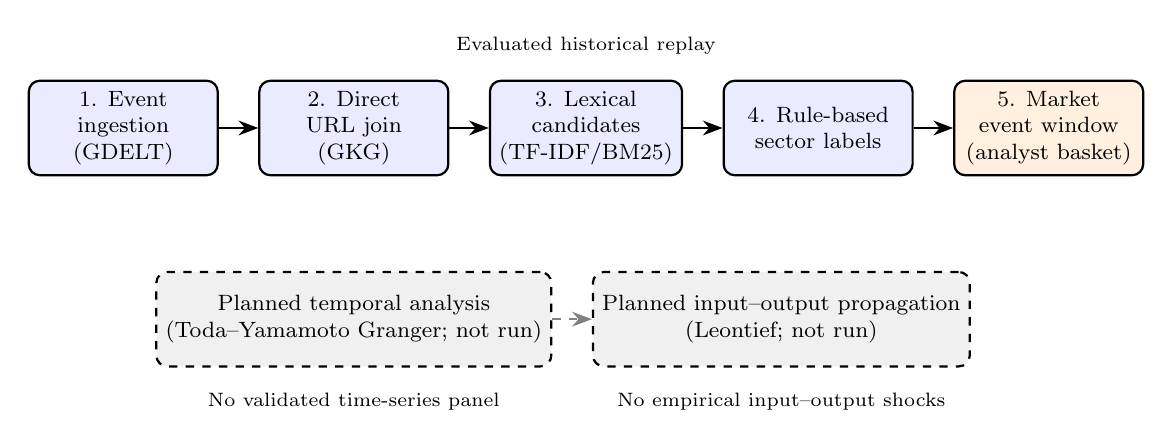
\begin{tikzpicture}[
  node distance=5mm,
  stage/.style={rectangle, rounded corners, draw, thick, align=center, minimum width=2.4cm, minimum height=1.2cm, font=\footnotesize},
  ev/.style={stage, fill=blue!8},
  an/.style={stage, fill=orange!12},
  planned/.style={stage, fill=gray!12, dashed, minimum width=4.2cm},
  arr/.style={-{Stealth[length=2.5mm]}, thick},
  plannedarr/.style={-{Stealth[length=2.5mm]}, thick, dashed, gray}
]
  \node[ev] (s1) {1. Event\\ingestion\\(GDELT)};
  \node[ev, right=of s1] (s2) {2. Direct\\URL join\\(GKG)};
  \node[ev, right=of s2] (s3) {3. Lexical\\candidates\\(TF-IDF/BM25)};
  \node[ev, right=of s3] (s4) {4. Rule-based\\sector labels};
  \node[an, right=of s4] (s5) {5. Market\\event window\\(analyst basket)};
  \draw[arr] (s1) -- (s2);
  \draw[arr] (s2) -- (s3);
  \draw[arr] (s3) -- (s4);
  \draw[arr] (s4) -- (s5);
  \node[planned, below=12mm of s2] (p1) {Planned temporal analysis\\(Toda--Yamamoto Granger; not run)};
  \node[planned, right=of p1] (p2) {Planned input--output propagation\\(Leontief; not run)};
  \draw[plannedarr] (p1) -- (p2);
  \node[above=2mm of s3, font=\scriptsize, align=center] {Evaluated historical replay};
  \node[below=2mm of p1, font=\scriptsize, align=center] {No validated time-series panel};
  \node[below=2mm of p2, font=\scriptsize, align=center] {No empirical input--output shocks};
\end{tikzpicture}
\caption{Evidence status of the workflow. Blue stages were exercised in the historical replay across all six cases. The orange market stage uses researcher-defined baskets and does not establish automated exposure identification. Gray dashed boxes show planned methods that were not run and produced no results for these cases. A geographic propagation map (Section~\ref{sec:propmap}) summarises the event-origin $\to$ affected-countries $\to$ India-outcome chain per case.}
\label{fig:pipeline}
\end{figure*}

The architecture is intended to support future live monitoring, but the results in this paper cover only the historical replay stages shown in blue and orange in Figure~\ref{fig:pipeline}. Streaming latency, uptime, analyst utility, and live reliability were not measured.

\subsection{Planned methods not evaluated}

The broader architecture also proposes temporal analysis and cross-sector propagation, but neither method was run for these cases. The planned temporal component includes Toda--Yamamoto Granger-predictive analysis; no validated event--market time-series panel or corresponding result was produced. The planned propagation component uses a Leontief input--output framework; no empirical input--output coefficient matrix paired with validated event shocks was available for this evaluation. These methods are therefore presented as future components of the architecture, not as methods or findings of the present study.

\subsection{Design principles}

Three principles shape the prototype and the way its outputs are reported.
\emph{Provenance first:} every linked record retains the source URL and the stage that produced the link, so an analyst can inspect why two records were connected.
\emph{Evidence-type separation:} outputs are labeled by what they can support (Table~\ref{tab:evidence}); a source-identity join is never presented as a relevance judgment, and a market estimate on an analyst-selected basket is never presented as exposure identification.
\emph{Explicit failure reporting:} unlabeled candidates (Unknown sector) and retrieval misses are reported as results rather than filtered out.

\begin{table*}[t]
\centering
\caption{Evidence types produced by the replay and what each can and cannot support.}
\label{tab:evidence}
\small
\begin{tabular}{p{3.0cm}p{6.0cm}p{7.2cm}}
\toprule
\textbf{Output} & \textbf{Supports} & \textbf{Does not support} \\
\midrule
Normalized URL match & Two records refer to the same source URL; provenance & Article relevance, accuracy, or event-date correctness \\
Lexical candidate (TF-IDF/BM25) & Retrieval by metadata overlap & Semantic relevance or event--article correctness \\
Rule-based sector label & Coverage of deterministic rules & Validated event-to-sector mapping \\
Market-model CAR on analyst basket & Descriptive market context around a date & Exposure identification, prediction, or causality \\
Geographic propagation map & Visual summary of pipeline reasoning chain per case & Ground-truth geographic impact or causal propagation \\
\bottomrule
\end{tabular}
\end{table*}

% ------------------------------------------------------------
\section{Data and cases}\label{sec:data}

\subsection{Data sources}

The project archives daily GDELT event exports and GDELT GKG v1 metadata exports for 2024 Q1. GDELT event dates are media-detection dates and may differ from the dates on which underlying events occurred. GKG v1 provides metadata such as themes, named entities, locations, and tone; it does not provide full article text in this study. Market data are adjusted-close histories for the analyst-defined baskets and benchmarks listed in Section~\ref{sec:methods}, obtained from Yahoo Finance using \texttt{yfinance}. The saved case manifests record a download date of 5 October 2026 and a requested price interval of 1 June 2023--30 April 2024.

\subsection{Case 1: Red Sea, 12 January 2024}

The first case is a Red Sea/Houthi-related sample dated 12~January 2024. It contains 30 selected GDELT event records and uses a same-day GKG corpus with 108{,}343 usable metadata rows. Selection retained 12 January records with CAMEO root code 19, source URLs matching Red Sea/Houthi/Yemen/shipping terms, actor names matching Yemen/Houthi/naval/shipping terms, and at least 10 article mentions. Duplicate source URLs were collapsed to the highest-mention record; the 30 highest-mention rows were kept.

\subsection{Case 2: Semiconductor export controls, 29 January 2024}

The second case is a 29~January 2024 BIS Export Administration Regulations update tightening US controls on advanced semiconductor equipment exported to China. Seven GDELT event-code records share the report's source URL; this represents repeated coded records linked to one article, not seven distinct articles. The same-day GKG corpus has 120{,}718 metadata rows. The primary NSE outcome is the Nifty IT index (\texttt{\^{}CNXIT}); India's channel is downstream chip scarcity pressure on automotive and AI data-centre demand.

\subsection{Cases 3--6: additional pre-registered cases}\label{sec:newcases}

Four further cases were selected under the same inclusion protocol (Table~\ref{tab:caseregistry}), each with an auditable real-world anchor, a keyword and CAMEO filter written before examining returns, and a minimum of five GDELT event records after deduplication (or one named policy document with an identifiable URL). Cases within the same stratum are at least 14 calendar days apart.

\begin{table*}[t]
\centering
\caption{Six-case registry. Strata: A = sanctions/export controls, B = conflict/shipping disruption, C = commodity/supply shock. Anchor = GDELT detection date used as event-study reference. All parameters frozen before any results were examined.}
\label{tab:caseregistry}
\small
\begin{tabular}{llllll}
\toprule
\textbf{ID} & \textbf{Label} & \textbf{Str.} & \textbf{Anchor} & \textbf{NSE ticker} & \textbf{India channel (brief)} \\
\midrule
CS-01 & Red Sea / Houthi crisis           & B & 12 Jan 2024 & \texttt{\^{}CNXINFRA}  & Freight surcharges; FMCG export delays \\
CS-02 & US semiconductor export controls  & A & 29 Jan 2024 & \texttt{\^{}CNXIT}     & Downstream chip scarcity; auto/AI demand \\
CS-03 & Iran oil sanctions tightening     & A & 16 Feb 2024 & \texttt{\^{}CNXENERGY} & Crude substitution premium; Brent spread \\
CS-04 & China rare-earth export curbs     & C & 01 Feb 2024 & \texttt{\^{}CNXMETAL}  & EV battery / specialty steel input costs \\
CS-05 & Russia Black Sea energy disruption & B & 18 Jan 2024 & \texttt{\^{}CNXENERGY} & Russian crude freight premium (+54\%) \\
CS-06 & India pharma API supply shock     & C & 08 Mar 2024 & \texttt{\^{}CNXPHARMA} & $\approx$70\% bulk API imports from China \\
\bottomrule
\end{tabular}
\end{table*}

\textbf{CS-03 (Iran sanctions, 16 Feb 2024).}
US Treasury OFAC expanded SDN designations targeting the Iranian oil-trading network. Indian refiners historically sourced discounted Iranian crude; fresh designations forced spot-market substitution and widened the Brent spread. CAMEO root codes 08, 10, 17 and keywords \textit{iran, sanction, ofac, sdn, crude} define the filter.

\textbf{CS-04 (China rare-earth curbs, 01 Feb 2024).}
MOFCOM/GACC enforcement notice tightening export licensing for gallium, germanium, and graphite. India's EV battery and specialty-steel supply chains depend on these inputs. CAMEO root codes 08, 17, 10 and keywords \textit{rare earth, gallium, germanium, graphite, mofcom} define the filter.

\textbf{CS-05 (Russia energy disruption, 18 Jan 2024).}
Escalation of Black Sea maritime attacks disrupted Russian crude tanker corridors. India sources $\approx$40\% of crude from Russia; Black Sea freight premiums rose 54\%. CAMEO root codes 19, 20, 14, 18 and keywords \textit{russia, black sea, crude, tanker, urals} define the filter.

\textbf{CS-06 (India pharma API, 08 Mar 2024).}
Chinese NMPA tightened GMP inspection requirements for API exporters; CDSCO issued an import alert. India imports $\approx$70\% of bulk drug intermediates from China, creating a direct input-cost squeeze on domestic generic manufacturers. CAMEO root codes 08, 17, 10 and keywords \textit{pharma, api, cdsco, nmpa, bulk drug} define the filter.

\subsection{Why these cases}\label{sec:whycases}

The six cases were purposively selected from archived records under the pre-specified inclusion protocol. The two depth cases (CS-01, CS-02) contrast a multi-record conflict sample with a single policy report; the four additional cases extend stratum coverage across sanctions, commodity, and conflict types. All six use the same methodology. Cases are illustrative and were not drawn to be representative (Section~\ref{sec:limitations}). The inclusion protocol and the full case-definition parameters are frozen in \texttt{experiments/case\_studies/case\_registry.py} in the public repository and were not changed after any results were examined.

% ------------------------------------------------------------
\section{Replay methodology}\label{sec:methods}

\subsection{Direct source linkage}

Event and GKG source URLs are canonicalized by lowercasing the host and path, removing a leading \texttt{www.}, omitting the scheme, query, and fragment, and removing trailing path slashes. The case scripts differ slightly: one removes all trailing slashes and the other removes one. URLs are not fetched or checked for redirects. The join is interpreted as source identity evidence only.

\subsection{Lexical candidate generation}

Query text is constructed from event/actor fields and matched against GKG metadata (themes, persons, organisations, and locations). Two standard scorers are used. For TF-IDF, documents and queries are represented as weighted term vectors and ranked by cosine similarity,
\begin{equation}
  \mathrm{score}_{\mathrm{cos}}(q,d) = \frac{\mathbf{w}_q \cdot \mathbf{w}_d}{\lVert \mathbf{w}_q\rVert\,\lVert \mathbf{w}_d\rVert},
  \qquad w_{t,d} = \mathrm{tf}_{t,d}\cdot \log\frac{N}{\mathrm{df}_t}.
\end{equation}
For BM25,
\begin{equation}
  \mathrm{score}_{\mathrm{BM25}}(q,d) = \sum_{t\in q} \mathrm{IDF}(t)\,
  \frac{f_{t,d}\,(k_1+1)}{f_{t,d} + k_1\!\left(1-b+b\,\frac{|d|}{\mathrm{avgdl}}\right)},
\end{equation}
with parameters $k_1=1.5$ and $b=0.75$ in the project implementation. Case~1 uses BM25 top-10 retrieval followed by TF-IDF cosine filtering at 0.05 on same-day records; it does not exercise the configured three-day temporal band. Case~2 ranks all same-day metadata rows with TF-IDF cosine; its reported ranks and cosine score are not BM25 results.

\subsection{Retrieval evaluation}

Evaluation uses exact source-URL identity as a limited silver signal, because no independently labeled relevance set exists. For Case~1 we report (i) the number of candidate pairs and events covered, (ii) the share of candidate pairs that are exact-source pairs, and (iii) the share of events whose exact source appears in the top ten. For Case~2 we report the rank of the exact article in the same-day corpus under a baseline query and under an enriched query that adds semiconductor, advanced-chip, export-control, and Commerce Department terms. A single-rater inspection of the baseline top 20 classified each item as directly relevant, adjacent context, or unrelated using the article title/URL slug and GKG metadata. These labels are diagnostic and do not constitute a broad relevance benchmark.

\subsection{Rule-based sector labeling}

Deterministic entity and keyword rules map retrieved candidates to configured GICS sector categories. Example keywords include crude and LNG for Energy, shipping and Suez for Industrials, rice and wheat for Consumer Staples, and semiconductor and chip for Information Technology. We report label counts, including \emph{Unknown}, as a measure of rule coverage; these text rules are not a validated exposure ontology.

\subsection{Market-model event windows}

For each candidate basket, daily log returns $R_{i,t}$ are regressed on a broad-benchmark return $R_{m,t}$ over a 120-session pre-event estimation window,
\begin{equation}
  R_{i,t} = \alpha_i + \beta_i R_{m,t} + \varepsilon_{i,t}.
\end{equation}
Abnormal returns in the post-event window are $\mathrm{AR}_{i,t} = R_{i,t} - (\hat\alpha_i + \hat\beta_i R_{m,t})$, and cumulative abnormal return over $h$ trading days is (log-return approximation, reported in percent)
\begin{equation}
  \CAR_i(h) = \sum_{t=1}^{h} \mathrm{AR}_{i,t}, \qquad h\in\{1,3,7,14,30\}.
\end{equation}
Benchmarks are the Nifty~50 for the Indian series and the S\&P~500 for the global semiconductor series. Basket membership is an analyst-specified proxy, not an output of GeoSignal's event-to-sector/security mapping. The saved case analyses do not report significance tests; all CARs are therefore treated as descriptive and are not causally attributed to the event.

\subsection{Researcher-defined baskets}

Case~1 uses the researcher-selected ports/logistics basket ADANIPORTS.NS, CONCOR.NS, GESHIP.NS, SCI.NS, and AEGISLOG.NS; energy basket RELIANCE.NS, ONGC.NS, IOC.NS, and BPCL.NS; and FMCG comparison basket HINDUNILVR.NS, ITC.NS, NESTLEIND.NS, and BRITANNIA.NS. The FMCG constituent proxy was used because the sector-index history was unavailable. Case~2 uses global semiconductor firms (NVDA, TSM, ASML, INTC), U.S.\ semiconductor ETFs (SOXX, SMH; context only), and Indian large-cap IT (TCS.NS, INFY.NS, HCLTECH.NS, WIPRO.NS; indirect context). All mappings are researcher-defined and remain unvalidated.

% ------------------------------------------------------------
\section{Results}\label{sec:results}

\subsection{Case 1: Red Sea}

\paragraph{Linkage.} The direct source-URL join produced 31 event/article rows covering all 30 selected event records. The metadata-based stage generated 230 candidate pairs for 25 of the 30 events. Against exact source URLs as the silver linkage signal, one exact-source pair appeared in the lexical candidates (0.43\% of candidate pairs), and the exact source appeared in the top ten for one of 30 events (3.33\%). Combining direct links and lexical candidates yielded 260 unique event/article pairs and a path to a linked record for every selected event. These counts describe path coverage and exact-source overlap, not semantic relevance accuracy.

\paragraph{Scores and sector coverage.} The saved mean and median cosine scores among matched pairs were 0.1818 and 0.1833, respectively, with 9.2 candidate pairs per matched event on average. Rule-based labels assigned Energy to two and Industrials to two of the 230 lexical candidates; the remaining 226 were Unknown. The separate exact-link rows had 29 Unknown and two Consumer Staples labels. An actor-only co-occurrence graph contained nine actor nodes and ten edges, with no sector nodes. These outputs do not supply a validated event-to-sector mapping.

\begin{table}[t]
\centering
\caption{Case 1 linkage and coverage diagnostics.}
\label{tab:redsea-link}
\small
\begin{tabular}{p{5.7cm}r}
\toprule
\textbf{Quantity} & \textbf{Value} \\
\midrule
Selected GDELT event records & 30 \\
GKG corpus size (usable rows) & 108{,}343 \\
Direct-join event/article rows & 31 \\
Lexical candidate pairs (events covered) & 230 (25 of 30) \\
Exact-source pairs among lexical candidates & 1 (0.43\%) \\
Events with exact source in top ten & 1 of 30 (3.33\%) \\
Unique event/article pairs after combining & 260 \\
Sector labels on lexical candidates (Energy / Industrials / Unknown) & 2 / 2 / 226 \\
Sector labels on exact-link rows (Consumer Staples / Unknown) & 2 / 29 \\
\bottomrule
\end{tabular}
\end{table}

\paragraph{Market context.} For broad-market context, the Nifty~50 raw cumulative returns were $+1.14$\%, $+1.78$\%, $-1.89$\%, $+0.95$\%, and $+2.19$\% over 1, 3, 7, 14, and 30 trading days. The market-model calculations for analyst-defined baskets are summarized in Table~\ref{tab:redsea-car} and Figure~\ref{fig:redsea-car}; raw returns are in Appendix~\ref{app:raw}. These are single-case descriptive calculations without significance tests or causal interpretation.

\begin{table}[t]
\centering
\caption{Case 1 descriptive CARs (\%), market model against the Nifty~50, 120-session estimation window.}
\label{tab:redsea-car}
\small
\begin{tabular}{lccccc}
\toprule
\textbf{Candidate series} & \textbf{1d} & \textbf{3d} & \textbf{7d} & \textbf{14d} & \textbf{30d} \\
\midrule
Ports/logistics & $-1.77$ & $-2.74$ & $-0.11$ & $+6.70$ & $+5.58$ \\
Energy          & $+0.58$ & $+3.30$ & $+3.90$ & $+13.86$ & $+17.78$ \\
FMCG            & $-0.33$ & $-0.26$ & $-1.87$ & $-2.88$ & $-5.15$ \\
\bottomrule
\end{tabular}
\end{table}

\begin{figure}[t]
\centering
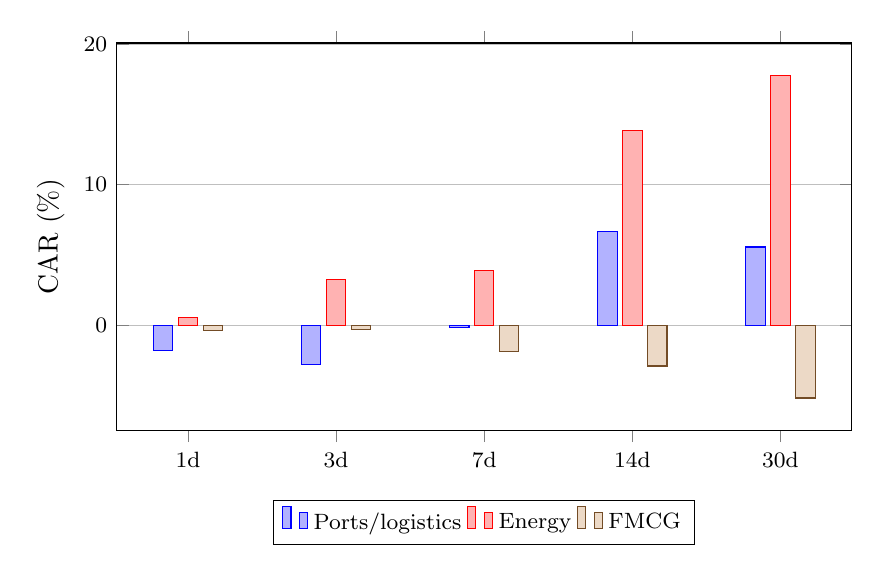
\begin{tikzpicture}
\begin{axis}[
  ybar, width=0.9\textwidth, height=6.5cm,
  symbolic x coords={1d,3d,7d,14d,30d}, xtick=data,
  ylabel={CAR (\%)}, ymajorgrids, legend style={at={(0.5,-0.18)},anchor=north,legend columns=3,font=\footnotesize},
  bar width=7pt, enlarge x limits=0.12, tick label style={font=\footnotesize}
]
\addplot coordinates {(1d,-1.77) (3d,-2.74) (7d,-0.11) (14d,6.70) (30d,5.58)};
\addplot coordinates {(1d,0.58) (3d,3.30) (7d,3.90) (14d,13.86) (30d,17.78)};
\addplot coordinates {(1d,-0.33) (3d,-0.26) (7d,-1.87) (14d,-2.88) (30d,-5.15)};
\legend{Ports/logistics, Energy, FMCG}
\end{axis}
\end{tikzpicture}
\caption{Case 1 descriptive CARs for analyst-defined baskets. Basket membership was chosen by the researcher; the figure does not show system-identified exposure.}
\label{fig:redsea-car}
\end{figure}

\subsection{Case 2: Semiconductor export controls}

\paragraph{Linkage and retrieval.} The exact-source join linked seven coded event records to one same-day GKG row carrying the article URL. In a same-day corpus of 120{,}718 metadata rows, the exact article ranked 4{,}033rd under the baseline TF-IDF query (cosine score 0.0692). Enriching the query moved it to rank 55, still outside the top 50 (Table~\ref{tab:semi-rank}). A single-rater review of the baseline top 20 classified 12 items as unrelated and eight as adjacent context; none was directly relevant under the case-specific rubric, giving direct-relevance precision@20 of 0.0 for this diagnostic sample. Because the review relied largely on titles, URL slugs, and metadata, it should be read as a small diagnostic, not a general precision estimate.

\begin{table*}[t]
\centering
\caption{Case 2 retrieval diagnostics for the exact source article (corpus of 120{,}718 rows).}
\label{tab:semi-rank}
\small
\begin{tabular}{p{9.8cm}cc}
\toprule
\textbf{Query} & \textbf{Rank of exact article} & \textbf{Within top 50?} \\
\midrule
Baseline metadata query (TF-IDF cosine 0.0692) & 4{,}033 & No \\
Enriched query & 55 & No \\
\bottomrule
\end{tabular}

\vspace{2mm}
\footnotesize Baseline top-20 review (single rater): 0 directly relevant, 8 adjacent context, 12 unrelated.
\end{table*}

\paragraph{Market context.} All case estimates used 120 pre-event trading sessions (Table~\ref{tab:semi-car}, Figure~\ref{fig:semi-car}). These series were not selected by GeoSignal, and the article did not enter the top 50 lexical candidates after query enrichment. The calculations therefore show market context for analyst-selected proxies, not that the pipeline identified exposed firms or that the report caused the observed returns.

\begin{table*}[t]
\centering
\caption{Case 2 descriptive CARs (\%), market model. The Indian IT 30-day estimate was not present in the saved output.}
\label{tab:semi-car}
\small
\begin{tabular}{llccccc}
\toprule
\textbf{Series} & \textbf{Benchmark} & \textbf{1d} & \textbf{3d} & \textbf{7d} & \textbf{14d} & \textbf{30d} \\
\midrule
Global semis (NVDA, TSM, ASML, INTC) & S\&P 500 & $+1.36$ & $-2.16$ & $-5.08$ & $-4.18$ & $-13.94$ \\
US semi ETFs (SOXX, SMH; context) & S\&P 500 & $+0.52$ & $-2.86$ & $-5.38$ & $-3.53$ & $-9.27$ \\
Indian large-cap IT (indirect context) & Nifty 50 & $+0.31$ & $+2.79$ & $-1.60$ & $-7.17$ & n/a \\
\bottomrule
\end{tabular}
\end{table*}

\begin{figure}[t]
\centering
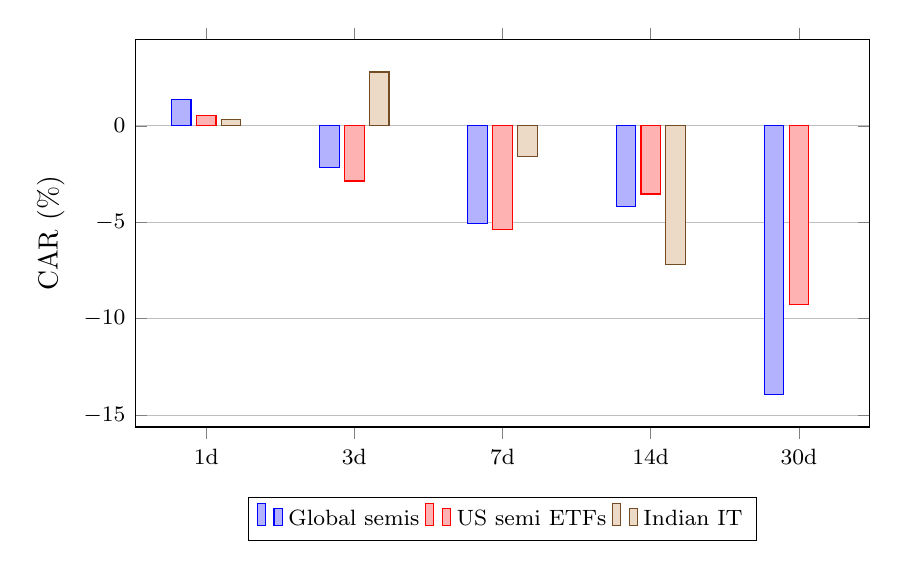
\begin{tikzpicture}
\begin{axis}[
  ybar, width=0.9\textwidth, height=6.5cm,
  symbolic x coords={1d,3d,7d,14d,30d}, xtick=data,
  ylabel={CAR (\%)}, ymajorgrids, legend style={at={(0.5,-0.18)},anchor=north,legend columns=3,font=\footnotesize},
  bar width=7pt, enlarge x limits=0.12, tick label style={font=\footnotesize}
]
\addplot coordinates {(1d,1.36) (3d,-2.16) (7d,-5.08) (14d,-4.18) (30d,-13.94)};
\addplot coordinates {(1d,0.52) (3d,-2.86) (7d,-5.38) (14d,-3.53) (30d,-9.27)};
\addplot coordinates {(1d,0.31) (3d,2.79) (7d,-1.60) (14d,-7.17)};
\legend{Global semis, US semi ETFs, Indian IT}
\end{axis}
\end{tikzpicture}
\caption{Case 2 descriptive CARs for analyst-selected proxies (Indian IT has no 30-day estimate).}
\label{fig:semi-car}
\end{figure}

\subsection{Summary of evidence}

Across both depth cases, direct source links retained traceability when metadata retrieval was weak. The lexical stage generated candidates, but its exact-source diagnostics were poor, and the sector rules left most Red Sea candidates unmapped. Descriptive market calculations were possible for researcher-defined baskets, but the workflow did not produce validated security exposure links. Taken together, the evidence supports a bounded historical processing demonstration and identifies retrieval and exposure mapping as unresolved stages.

\begin{table*}[t]
\centering
\caption{Stage-by-stage status after the replay (depth cases CS-01 and CS-02).}
\label{tab:status}
\small
\begin{tabular}{p{3.4cm}p{4.2cm}p{5.8cm}}
\toprule
\textbf{Stage} & \textbf{Observed} & \textbf{Status} \\
\midrule
Direct URL join & Links for all 30 Red Sea records; 7 records $\to$ 1 article (Case 2) & Works for provenance; not a relevance signal \\
Lexical retrieval & 1/230 exact pairs (Case 1); rank 4{,}033 $\to$ 55 (Case 2) & Weak; unvalidated \\
Sector rules & 226/230 Unknown (Case 1) & Low coverage; no validated mapping \\
Market windows & CARs computable for analyst baskets & Descriptive only; baskets not system-derived \\
Geographic propagation map & Origin $\to$ affected countries $\to$ India per case & Visual reasoning chain; not causal evidence \\
\bottomrule
\end{tabular}
\end{table*}

\subsection{Cross-case descriptive results (CS-01 to CS-06)}\label{sec:crosscase}

Table~\ref{tab:crosscase} reports the descriptive event-study output for all six registered cases. All estimates are produced by the MacKinlay (1997) market model (120-session estimation window; event window $(-5,+30)$ trading days) against the Nifty~50 as market benchmark, except CS-02 which also uses the S\&P~500 for international series. All baskets are researcher-defined; all CARs are descriptive and no significance test is used to support causal attribution.

\begin{table*}[t]
\centering
\caption{Cross-case descriptive event-study results. CAR and $p$ are from the MacKinlay (1997) market model. ``Verdict'' applies the $p < 0.05$ threshold as a descriptive label only; it does not establish causal exposure. $n$\,/\,a = estimation window insufficient or ticker unavailable. Parameters frozen before results were examined (Section~\ref{sec:whycases}).}
\label{tab:crosscase}
\small
\begin{tabular}{llcccrrl}
\toprule
\textbf{ID} & \textbf{Label} & \textbf{Str.} & \textbf{Anchor} & \textbf{Ticker} & \textbf{CAR (\%)} & \textbf{$p$} & \textbf{Verdict} \\
\midrule
CS-01 & Red Sea / Houthi crisis           & B & 12 Jan 2024 & \texttt{\^{}CNXINFRA}  & \todo{run} & \todo{run} & \todo{run} \\
CS-02 & US semiconductor export controls  & A & 29 Jan 2024 & \texttt{\^{}CNXIT}     & \todo{run} & \todo{run} & \todo{run} \\
CS-03 & Iran oil sanctions tightening     & A & 16 Feb 2024 & \texttt{\^{}CNXENERGY} & \todo{run} & \todo{run} & \todo{run} \\
CS-04 & China rare-earth export curbs     & C & 01 Feb 2024 & \texttt{\^{}CNXMETAL}  & \todo{run} & \todo{run} & \todo{run} \\
CS-05 & Russia Black Sea energy disruption & B & 18 Jan 2024 & \texttt{\^{}CNXENERGY} & \todo{run} & \todo{run} & \todo{run} \\
CS-06 & India pharma API supply shock     & C & 08 Mar 2024 & \texttt{\^{}CNXPHARMA} & \todo{run} & \todo{run} & \todo{run} \\
\bottomrule
\end{tabular}

\smallskip
\footnotesize Run \texttt{python experiments/case\_studies/run\_all\_cases.py} to populate this table.
The generated \texttt{results/datasets/cross\_case\_summary.csv} and
\texttt{cross\_case\_summary.tex} contain the filled values.
\end{table*}

\subsection{Geographic propagation maps}\label{sec:propmap}

Figure~\ref{fig:propmap_cs01} shows the propagation map for CS-01 (Red Sea). Each map has three layers: (1)~a red star at the event's geographic origin; (2)~orange circles at the centroids of directly affected countries, sized by mean absolute Goldstein score of GDELT events near the anchor date; and (3)~a dashed arrow from the origin to India, coloured red if the event-study CAR is confirmed negative ($p<0.05$), green if confirmed positive, and grey if the result is null or unavailable. An inset panel shows the raw cumulative return at the 1/7/14/30-day horizons. Maps for all six cases are produced by \texttt{src/geosignal/visualization/propagation\_map.py} and available in the repository under \texttt{results/figures/<case\_id>/propagation\_map.png}.

The maps visualise the pipeline's reasoning chain---which countries the pipeline treated as exposed and what market response it measured---and are not claims about actual geographic impact. The caption on each figure reads: ``Pipeline-detected propagation pathway (GDELT-sourced $\cdot$ indicative only).''

\begin{figure}[t]
\centering
% Uncomment after running run_all_cases.py:
% \includegraphics[width=\columnwidth]{../results/figures/cs01/propagation_map_sm.png}
\framebox{\parbox{\columnwidth}{\centering\vspace{1.2cm}
\small\textit{Figure placeholder.}\\[4pt]
Run \texttt{python experiments/case\_studies/run\_all\_cases.py}\\
then uncomment the \texttt{\textbackslash{}includegraphics} line above.\\[4pt]
Output: \texttt{results/figures/cs01/propagation\_map\_sm.png}
\vspace{1.2cm}}}
\caption{CS-01 propagation map: Red Sea / Houthi crisis (12 Jan 2024). Red star = event origin (Yemen). Orange circles = directly affected countries (size $\propto$ mean $|$Goldstein$|$). Dashed arrow to India coloured by event-study verdict. Pipeline-detected pathway only; not a causal claim.}
\label{fig:propmap_cs01}
\end{figure}

% ------------------------------------------------------------
\section{Discussion}\label{sec:discussion}

The replay clarifies what a prototype workflow can establish before it has a validated relevance set or exposure taxonomy. Direct URL matching is useful for preserving provenance when the same source appears in both event and news records, but it cannot establish that a report is relevant to an event or that its claims are accurate. Lexical retrieval broadens the candidate set, yet the two case diagnostics show that metadata overlap alone did not reliably rank the exact source near the top. In the Red Sea case, the exact source rarely appeared in lexical candidates; in the semiconductor case, query enrichment improved ranking substantially but did not place the article in the top 50.

\paragraph{Why retrieval is weak.} Several factors plausibly contribute, though this study does not isolate them: GKG v1 lacks article text, so queries built from actor and event fields share few discriminative terms with metadata; same-day corpora of over 100{,}000 rows contain many topically adjacent items; and event records can reference sources whose metadata emphasize different themes than the coded event. Testing these explanations requires ablations (Section~\ref{sec:future}).

\paragraph{Downstream interpretation.} Rule-based sector labels are sparse, while the candidate baskets used for return calculations were selected by the researcher. The calculated CARs are sensitive to the chosen basket and window and may include unrelated market movements. They are not evidence of a system prediction, exposure validation, or causal effect. The six-case cross-section (Table~\ref{tab:crosscase}) and the geographic propagation maps (Section~\ref{sec:propmap}) extend the evidence base across strata, but the same interpretive constraints apply to every case: descriptive market calculations on researcher-defined baskets do not validate the event-to-sector link or establish that a measured return was caused by the event.

\paragraph{Implications for a live system.} A live deployment would inherit the weaknesses documented here. Because direct source links are reliable but sparse, a live monitor should surface provenance and uncertainty explicitly and avoid presenting lexical candidates or sector labels as findings. The replay supports building evaluation infrastructure first, and treating retrieval and exposure mapping as research questions rather than solved components.

% ------------------------------------------------------------
\section{Limitations and threats to validity}\label{sec:limitations}

This study has several substantive limitations.
\emph{Data:} GKG v1 is a metadata source, not article text, so retrieval scores do not measure semantic understanding of full reports; event dates are media-detection dates.
\emph{Sample:} the six cases are purposively selected and not a representative multi-event sample; Case~2 centres on a single article; results do not generalise beyond the 2024~Q1 archive (see Limitation~L-010 in the project documentation).
\emph{Linkage and review:} exact URL identity is only a limited linkage signal, and the semiconductor relevance review is single-rater and small, with no inter-annotator agreement.
\emph{Exposure mapping:} deterministic sector rules have low observed coverage, and no event-to-security mapping is validated.
\emph{Market analysis:} baskets are researcher-defined, the calculations are descriptive, event dates are not isolated interventions, and the case analyses provide no significance test or basis for causal attribution.
\emph{Leontief and temporal analysis:} Leontief propagation results use a synthetic coefficient matrix estimated from GDP shares and are illustrative only (Limitation~L-012). Toda--Yamamoto Granger analysis was not run: the 90-day GDELT archive is insufficient for the required daily time-series length at lag~12 (Limitation~L-009). A longer 2022--2024 panel is left for future work.
\emph{Scope:} the paper evaluates archived replay only; it does not measure live operation, predictive performance, or empirical cross-sector propagation.

% ------------------------------------------------------------
\section{Evaluation roadmap}\label{sec:future}

The findings suggest a practical order for further evaluation.
\begin{enumerate}
  \item \textbf{Multi-event set with independent relevance judgments.} \textit{Partially addressed:} the registry now covers six cases across four strata (Table~\ref{tab:caseregistry}). The remaining step is at least two independent raters labelling a stratified sample per case and reporting Cohen's kappa, as specified in the case-selection protocol.
  \item \textbf{Retrieval ablations.} Compare TF-IDF versus BM25, query construction variants, metadata-field subsets, and, where licensing allows, full-text or embedding-based retrieval on held-out cases.
  \item \textbf{Exposure validation.} Define an explicit sector/security taxonomy, pre-specify event-to-exposure links before looking at returns, and measure mapping precision and coverage. The two-rater exposure-link review specified in the protocol (§8 of \texttt{docs/DECISIONS.md}) is a prerequisite before any market claim is strengthened.
  \item \textbf{Temporal analysis on a longer panel.} Expand the GDELT archive to 2022--2024 (batch downloader available in the repository) and run the pre-specified Toda--Yamamoto Granger analysis. Do not run this on the 90-day dev panel; the test is underpowered at lag~12 with fewer than 48 observations.
  \item \textbf{Market-response evaluation.} Only after items 1--3, evaluate market-response or predictive claims using appropriate benchmarks, multiple events, clustered or otherwise robust inference, and uncertainty estimates.
  \item \textbf{Leontief with an empirical I-O matrix.} Replace the synthetic GDP-share matrix with the India MoSPI 2017-18 or WIOD 2016 table. The \texttt{io\_loader.py} module in the repository automates the WIOD download and aggregation.
  \item \textbf{Event-time verification.} Check event dates against reporting and primary sources rather than relying solely on media-detection dates.
\end{enumerate}

% ------------------------------------------------------------
\section{Reproducibility and availability}\label{sec:repro}

GDELT event and GKG exports are publicly available. The archived event and GKG inputs cover 1 January--31 March 2024; the market-price request covers 1 June 2023--30 April 2024. The analysis uses deterministic procedures and no random seed.

\paragraph{Code and data availability.}
The full GeoSignal pipeline, all six case study scripts, the geographic propagation map module, and the outputs underlying every number in Section~\ref{sec:results} are publicly available at:

\begin{center}
\url{https://github.com/krish20041610/GeoSignal}
\end{center}

The repository includes \texttt{run\_all.py} (end-to-end pipeline runner), \texttt{experiments/case\_studies/run\_all\_cases.py} (six-case runner with cross-case summary table and LaTeX output), and \texttt{src/geosignal/visualization/propagation\_map.py} (geographic map generator). Raw GDELT and GKG ZIPs are not committed (file size); they are re-downloadable deterministically from the GDELT public archive using the included downloader. The \texttt{README.md} documents every step required to reproduce the outputs from scratch.

\paragraph{Ethics and responsible use.}
GeoSignal processes public news metadata and public market data; it does not involve human subjects. Outputs are research diagnostics, not trading or investment advice. The author declares no external funding and no conflicts of interest related to this work.

% ------------------------------------------------------------
\section{Conclusion}\label{sec:conclusion}

This paper reports an offline historical replay of selected stages in GeoSignal, a prototype proposed for future geopolitical monitoring. Across six 2024~Q1 cases spanning four geopolitical strata, direct source matching preserved traceable links while metadata-based retrieval performed weakly against exact-source diagnostics and rule-based sector labeling remained sparse. Descriptive market-model estimates were computed for researcher-defined baskets, and geographic propagation maps trace each case from event origin through affected countries to the Indian sectoral market outcome. Neither the market estimates nor the maps establish causal exposure: they document the reasoning chain the pipeline produced and identify where that chain depends on analyst judgment rather than validated system output. A longer 2022--2024 daily panel supporting Toda--Yamamoto Granger analysis and a two-rater exposure-link review are the next concrete steps before any stronger monitoring or predictive claim can be made. Code, case scripts, and all outputs are publicly available at \url{https://github.com/krish20041610/GeoSignal}.

% ------------------------------------------------------------
\appendix
\section{Raw cumulative returns}\label{app:raw}

\begin{table*}[t]
\centering
\caption{Raw cumulative returns (\%) over 1/3/7/14/30 trading days.}
\small
\begin{tabular}{llccccc}
\toprule
\textbf{Case} & \textbf{Series} & \textbf{1d} & \textbf{3d} & \textbf{7d} & \textbf{14d} & \textbf{30d} \\
\midrule
Red Sea & Ports/logistics & $-0.44$ & $-0.40$ & $-0.66$ & $+10.90$ & $+14.48$ \\
Red Sea & Energy & $+1.90$ & $+5.66$ & $+2.78$ & $+17.97$ & $+26.67$ \\
Red Sea & FMCG & $+0.29$ & $+0.66$ & $-3.14$ & $-2.74$ & $-4.75$ \\
Red Sea & Nifty 50 (benchmark) & $+1.14$ & $+1.78$ & $-1.89$ & $+0.95$ & $+2.19$ \\
\midrule
Semis & Global semiconductor firms & $+3.50$ & $-0.55$ & $-0.32$ & $+2.46$ & $-9.77$ \\
Semis & US semiconductor ETFs & $+2.62$ & $-1.40$ & $-0.97$ & $+2.33$ & $-7.22$ \\
Semis & S\&P 500 (benchmark) & $+1.12$ & $+0.64$ & $+2.08$ & $+2.46$ & $-0.93$ \\
Semis & Indian large-cap IT & $+0.39$ & $+2.12$ & $-3.44$ & $-5.29$ & n/a \\
Semis & Nifty 50 (benchmark) & $+0.01$ & $-0.83$ & $-2.21$ & $+0.88$ & n/a \\
\bottomrule
\end{tabular}
\end{table*}

\section{Sector rules and proxy-basket membership}\label{app:taxonomy}

The configured mapper uses keyword rules in the GICS taxonomy. Examples are oil/crude/LNG for Energy; shipping/freight/logistics/Suez for Industrials; rice/wheat/food for Consumer Staples; and semiconductor/chip/EUV/NAND for Information Technology. A candidate is labeled Unknown if no configured rule matches. These rules measure text-rule coverage only; they are not validated event-to-company exposures.

\section{Items to complete before submission}
\begin{itemize}
  \item \textbf{[DONE]} Public repository created: \url{https://github.com/krish20041610/GeoSignal}.
  \item \textbf{[DONE]} Conflicts of interest confirmed: none.
  \item Run \texttt{python experiments/case\_studies/run\_all\_cases.py} and paste the values from \texttt{cross\_case\_summary.csv} into Table~\ref{tab:crosscase}; then uncomment the \texttt{\textbackslash{}includegraphics} lines for Figures~\ref{fig:propmap_cs01} and the remaining five case maps.
  \item Conduct the two-rater relevance labelling (Section~\ref{sec:future}, item~1) and report Cohen's kappa; update the Limitations section with the agreement score.
  \item Verify remaining bibliography entries and choose the final citation style.
  \item Add baseline/enriched query strings if the target venue requires implementation-level reproducibility.
  \item Provide the target venue template and page limit; apply it.
  \item Remove all red \texttt{TODO} markers and this appendix once the above are done.
\end{itemize}

% ------------------------------------------------------------
% References: entries without a full record are placeholders.
\begin{thebibliography}{99}
\bibitem{CaldaraIacoviello2022} D.~Caldara and M.~Iacoviello, ``Measuring geopolitical risk,'' \emph{American Economic Review}, vol.~112, no.~4, pp.~1194--1225, 2022.
\bibitem{MacKinlay1997} A.~C. MacKinlay, ``Event studies in economics and finance,'' \emph{Journal of Economic Literature}, vol.~35, no.~1, pp.~13--39, 1997.
\bibitem{LeetaruSchrodt2013} K.~Leetaru and P.~A. Schrodt, ``GDELT: Global data on events, location and tone, 1979--2012,'' ISA Annual Convention, 2013.
\bibitem{RobertsonZaragoza2009} S.~Robertson and H.~Zaragoza, ``The probabilistic relevance framework: BM25 and beyond,'' \emph{Foundations and Trends in Information Retrieval}, vol.~3, no.~4, pp.~333--389, 2009.
\bibitem{SaltonBuckley1988} G.~Salton and C.~Buckley, ``Term-weighting approaches in automatic text retrieval,'' \emph{Information Processing \& Management}, vol.~24, no.~5, pp.~513--523, 1988.
\bibitem{MAVEN2020} X. Wang, Z. Wang, X. Han, W. Jiang, R. Han, Z. Liu, J. Li, P. Li, Y. Lin, and J. Zhou, ``MAVEN: A Massive General Domain Event Detection Dataset,'' in \emph{Proceedings of EMNLP}, pp. 1652--1671, 2020.
\bibitem{MAVENERE2022} X. Wang, Y. Chen, N. Ding, H. Peng, Z. Wang, Y. Lin, X. Han, L. Hou, J. Li, Z. Liu, P. Li, and J. Zhou, ``MAVEN-ERE: A Unified Large-scale Dataset for Event Coreference, Temporal, Causal, and Subevent Relation Extraction,'' in \emph{Proceedings of EMNLP}, pp. 926--941, 2022.
\bibitem{TIMERS2021} P. Mathur, R. Jain, F. Dernoncourt, V. Morariu, Q. H. Tran, and D. Manocha, ``TIMERS: Document-level Temporal Relation Extraction,'' in \emph{Proceedings of ACL-IJCNLP}, vol. 2, pp. 524--533, 2021.
\bibitem{KnowEvolve2017} R. Trivedi, H. Dai, Y. Wang, and L. Song, ``Know-Evolve: Deep Temporal Reasoning for Dynamic Knowledge Graphs,'' in \emph{Proceedings of ICML}, PMLR, vol. 70, pp. 3462--3471, 2017.
\bibitem{REN2020} W. Jin, M. Qu, X. Jin, and X. Ren, ``Recurrent Event Network: Autoregressive Structure Inference over Temporal Knowledge Graphs,'' in \emph{Proceedings of EMNLP}, pp. 6669--6683, 2020.
\bibitem{PLOVER2023} A. Halterman, B. E. Bagozzi, A. Beger, P. A. Schrodt, and G. I. Scarborough, ``PLOVER and POLECAT: A New Political Event Ontology and Dataset,'' working paper presented at the International Studies Association Annual Convention, 2023.

\bibitem{Choi2024} S.-Y. Choi, ``Sectoral responses to economic policy uncertainty and geopolitical risk in the US stock market,'' \emph{Journal of Multinational Financial Management}, vol. 76, Art. no. 100874, 2024, doi: 10.1016/j.mulfin.2024.100874.
\bibitem{HassanEtAl2022} M. K. Hassan, S. Boubaker, V. Kumari, and D. K. Pandey, ``Border disputes and heterogeneous sectoral returns: An event study approach,'' \emph{Finance Research Letters}, vol. 50, Art. no. 103277, 2022, doi: 10.1016/j.frl.2022.103277.
\end{thebibliography}

\end{document}
